% !TEX root =  main.tex
\chapter{Customized Chapter}

This is a customized chapter.

\section{First section}

\hspace{\parindent} You may change the filename of this file as
long as you correspondingly change the filename stated in the
\verb+input{}+ line in the \verb+main.tex+.

\section{Including figures}

\hspace{\parindent} Figures can be added into your \LaTeX files
using the \verb+figure+ environment.  However, it is
\textbf{recommended} that you use \verb+.eps+ file format.  These
are encapsulated postscript files.  This can be easily done by
installing a postscript printer that outputs to a file (port is
FILE).  Ask your system administrator to install such a device for
producing \verb+eps+ files by simply printing it to that device.

Shown in Fig.~\ref{fig:sampleFig} is a figure created from
Excel\circledR. Note that the bounding box and page bounding box
should be adjusted well enough to show the correct field.
\begin{figure}[h]
  \centering %%used to center the figure
  %% The width option is used to rescale the figure into the proper
  %% fraction of the \columnwidth
  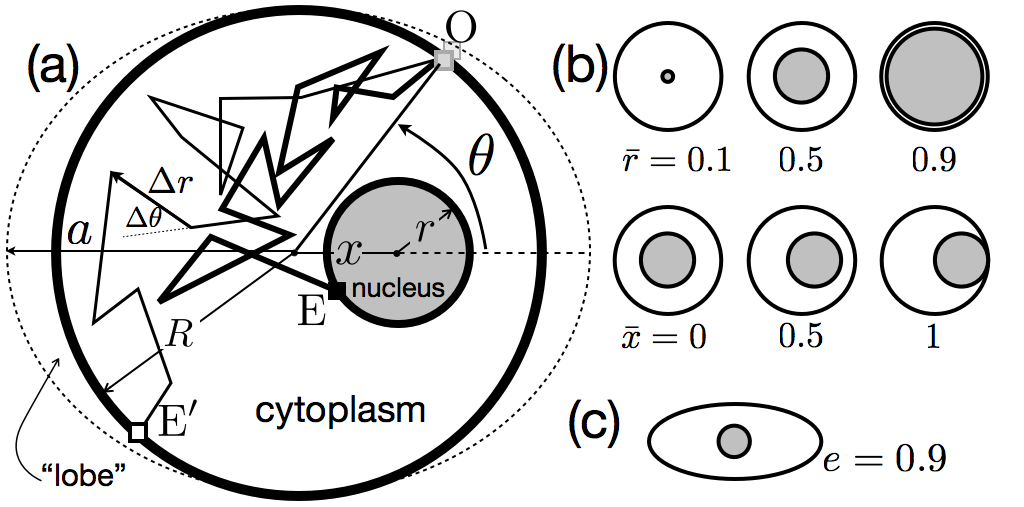
\includegraphics[width=0.8\columnwidth]{figures/model.png}\\
  \caption{
  A *.png file.
  }\label{fig:sampleFig}
\end{figure}

Please see the sample chapter on how the figure is included in the
\verb+tex+ files.
